
\subsection{Deep Learning Models of Sentence Salience}

\begin{frame}{Summarizer Architecture}
  \begin{center}
    \begin{tikzpicture}
      \node at (0.4,-.75) {Sentence 1};
      \node at (4.9,-.75) {Sentence 2};
      \node at (8.9,-.75) {Sentence 3};
      \node (w1) at (0,0) 
      {\large $\uncover<2->{\textsc{Enc}\left(}w^{(1)}_1,
         w^{(1)}_2, w^{(1)}_3\uncover<2->{\right)}$};

      \node (w2) at (4.5,0) 
      {\large $\uncover<2->{\textsc{Enc}\left(}w^{(2)}_1, 
         w^{(2)}_2, w^{(2)}_3\uncover<2->{ \right)}$};
      \node (w3) at (8.6,0) 
      {\large $\uncover<2->{\textsc{Enc}\left(}w^{(3)}_1, 
         w^{(3)}_2\uncover<2->{\right)}$};

      \node (s1) at (3,2) {\large $\uncover<3->{s_1}$};
      \node (s2) at (4,2) {\large $\uncover<3->{s_2}$};
      \node (s3) at (5,2) {\large $\uncover<3->{s_3}$};
      \uncover<3->{  
        \draw[->,thick] (w1.north) -- (s1.south); 
        \draw[->,thick] (w2.north) -- (s2.south);
        \draw[->,thick] (w3.north) -- (s3.south);
      }

      \uncover<4->{
        \node (ext) at (3.6,2) {\large $\textsc{Ext}\Big( 
        \quad\quad\quad\;\;\;\;\;\;\;\;\;\;\; \Big)$};
      }
      \uncover<5->{
        \node (y1) at (3,3.5) {\large $y_1$};
        \node (y2) at (4,3.5) {\large $y_2$};
        \node (y3) at (5,3.5) {\large $y_3$};
        \draw[->,thick] (s1.north) -- (y1.south);
        \draw[->,thick] (s2.north) -- (y2.south);
        \draw[->,thick] (s3.north) -- (y3.south);
      }

    \end{tikzpicture}
  \end{center}
\end{frame}


\begin{frame}{Sentence Encoders}
 \begin{columns}[t]
  \column{.32\textwidth}
   \centering
   Averaging Encoder\\~\\
   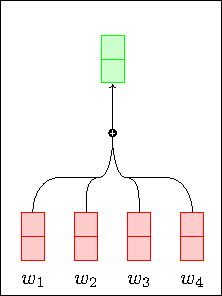
\includegraphics[]{images/section3/avg_encoder.pdf}\\
  \column{.32\textwidth}
   \centering
   RNN Encoder\\~\\
   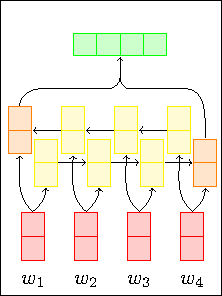
\includegraphics[]{images/section3/rnn_encoder.pdf}\\
  \column{.32\textwidth}
   \centering
   CNN Encoder\\~\\
   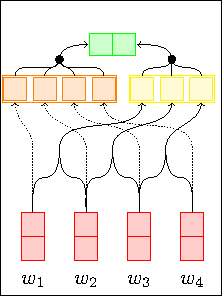
\includegraphics[]{images/section3/cnn_encoder.pdf}\\
 \end{columns}

~\\
We use pretrained (Wikipedia/Gigaword) Glove word embeddings.

\end{frame}
%
%\begin{frame}{Sentence Extractor}
%  \textbf{Previous Work}\\~\\
%  ~~ -- \textbf{Cheng and Lapata Extractor} ~~ seq2seq inspired architecture 
%                                               (Cheng and Lapata, 2016)\\
%  ~~ -- \textbf{SummaRunner Extractor} ~~ RNN inspired architecture with 
%                                          document and summary representations 
%                                          (Nallapati et al., 2016)\\
%  ~\\~\\
%  \textbf{Our Extractors}\\~\\
%  ~~ -- \alert<2>{\textbf{RNN Extractor}} ~~ Simplified version of SummaRunner \\
%  ~~ -- \textbf{Seq2Seq Extractor} ~~ seq2seq (with attention) inspired 
%                                      architecture \\
%\end{frame}


\begin{frame}{Sentence Extractors}
 \begin{columns}[t]
  \column{.4\textwidth}
  \only<1,2,4>{
   \centering
   SummaRunner Extractor\\
   (Nallapati et al. 2016)\\
   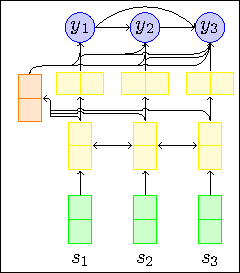
\includegraphics[scale=.65]{images/section3/sr_extractor.pdf}\\
   RNN Extractor (ours)\\
   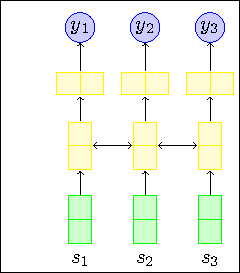
\includegraphics[scale=.65]{images/section3/rnn_extractor.pdf}
}
\only<3>{
    Cheng \& Lapata Model
    \begin{enumerate}
        \item Offset encoder/decoder inputs, no attention
        \item Complex interaction between previous extraction prediction and 
            decoder input.
    \end{enumerate}
    ~\\~\\
    Seq2Seq Model
    \begin{enumerate}
        \item Simple dot-product attention
        \item \textbf{(Conditionally) independent} extraction decisions
    \end{enumerate}
}
  \column{.6\textwidth}
  \only<1,3,4>{
   \centering
   Cheng \& Lapata Extractor\\
   (Cheng and Lapata, 2016)\\
   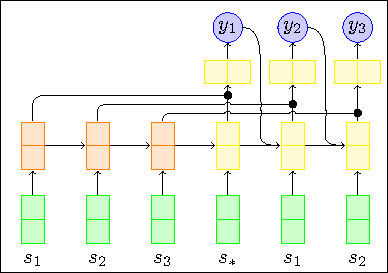
\includegraphics[scale=.65]{images/section3/cl_extractor.pdf}\\
   Seq2Seq Extractor (ours)\\
   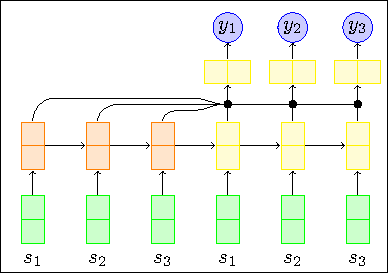
\includegraphics[scale=.65]{images/section3/s2s_extractor.pdf}
   }
   \only<2>{
        SummaRunner Model
        \begin{itemize}
        \item Internal representations of document similarity and summary novelty
        \item Explicit representation of position
        \item Complex dependencies between extraction decisions
        \end{itemize}
~\\
~\\
        RNN Model
        \begin{itemize}
            \item \sout{Internal representations of document similarity and summary novelty}
            \item \sout{Explicit representation of position}
            \item \textbf{(Conditionally) independent} extraction decisions
        \end{itemize}

   }
 \end{columns}

\end{frame}


\begin{frame}{Experiments}
%
    \alert<4>{\textbf{Main Experiment}}\\
    Evaluate encoder/extractor pairs using ROUGE-2 recall.\\
%
  \begin{columns}
    \begin{column}{0.3\textwidth}
    \uncover<5->{\textbf{Additional Experiments}}    
      \begin{itemize}
        \uncover<5->{\item \alert<5>{fine-tuned embeddings}}
        \uncover<6->{\item \alert<6>{word class ablations}}
        \uncover<7->{\item \alert<7>{sentence order shuffling}}
      \end{itemize}
    \end{column}
    \begin{column}{0.7\textwidth}
        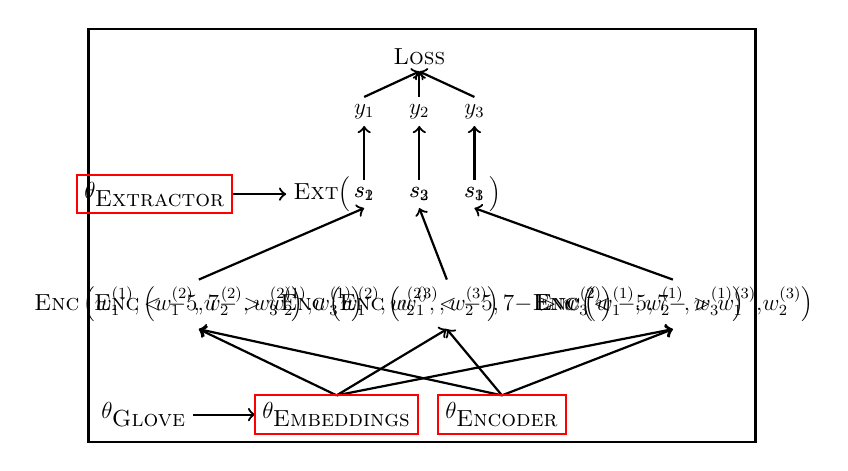
\begin{tikzpicture}[thick,scale=0.7, every node/.style={transform shape}]

  \draw[draw=black] (-2,5) rectangle (10.1,-2.5);

  \uncover<1-6>{
    \node (w1) at (0,0) 
      {\large $\textsc{Enc}\left(w^{(1)}_1,
       \uncover<-5,7->{w^{(1)}_2,} w^{(1)}_3\right)$};
    \node (w3) at (8.6,0) 
      {\large $\textsc{Enc}\left( \uncover<-5,7->{ w^{(3)}_1, }
       w^{(3)}_2 \right)$};
    \node (w2) at (4.5,0) 
      {\large $\textsc{Enc}\left(w^{(2)}_1, 
       w^{(2)}_2,\uncover<-5,7->{  w^{(2)}_3} \right)$};


  }
  
  \uncover<7>{
    \node (w21) at (0,0) 
      {\large $\textsc{Enc}\left(w^{(2)}_1, w^{(2)}_2,w^{(2)}_3 \right)$};
    \node (w13) at (8,0) 
      {\large $\textsc{Enc}\left(w^{(1)}_1, w^{(1)}_2, w^{(1)}_3\right)$};
    \node (w32) at (4,0) 
      {\large $\textsc{Enc}\left(w^{(3)}_1, w^{(3)}_2 \right)$};
  }





  \uncover<1-6>{
    \node (s1) at (3,2) {\large $s_1$};
    \node (s2) at (4,2) {\large $s_2$};
    \node (s3) at (5,2) {\large $s_3$};
  }
  \uncover<7>{
    \node (s13) at (5,2) {\large $s_1$};
    \node (s21) at (3,2) {\large $s_2$};
    \node (s32) at (4,2) {\large $s_3$};
  }


    \draw[->,thick] (w1.north) -- (s1.south); 
    \draw[->,thick] (w2.north) -- (s2.south);
    \draw[->,thick] (w3.north) -- (s3.south);

    \node (ext) at (3.6,2) {\large $\textsc{Ext}\Big( 
        \quad\quad\quad\;\;\;\;\;\;\;\;\;\;\; \Big)$};
\uncover<2->{
    \node (extp) at (-.8,2) {\large $\theta_\textsc{Extractor}$};
    \node (encp) at (5.5,-2) {\large $\theta_\textsc{Encoder}$};
    \draw[->,thick] (encp.north) -- (w1.south);
    \draw[->,thick] (encp.north) -- (w2.south);
    \draw[->,thick] (encp.north) -- (w3.south);
    \draw[->,thick] (extp.east) -- (ext.west);
}

\uncover<3->{
    \node (embp) at (2.5,-2) {\large $\theta_\textsc{Embeddings}$};
    \draw[->,thick] (embp.north) -- (w1.south);
    \draw[->,thick] (embp.north) -- (w2.south);
    \draw[->,thick] (embp.north) -- (w3.south);
}
\uncover<4->{
        \draw[draw=red] (extp.north east) rectangle (extp.south west);
       \draw[draw=red] (encp.north east) rectangle (encp.south west);
    \node (glovep) at (-1,-2) {\large $\theta_\textsc{Glove}$};
    \draw[->,thick] (glovep.east) -- (embp.west);

}
\uncover<5>{
        \draw[draw=red] (embp.north east) rectangle (embp.south west);
}
    \node (y1) at (3,3.5) {\large $y_1$};
    \node (y2) at (4,3.5) {\large $y_2$};
    \node (y3) at (5,3.5) {\large $y_3$};
    \draw[->,thick] (s1.north) -- (y1.south);
    \draw[->,thick] (s2.north) -- (y2.south);
    \draw[->,thick] (s3.north) -- (y3.south);

    \node (loss) at (4, 4.5) {\large \textsc{Loss}};
    \draw[->,thick] (y1.north) -- (loss.south);
    \draw[->,thick] (y2.north) -- (loss.south);
    \draw[->,thick] (y3.north) -- (loss.south);
 

%    \uncover<2->{   
 %      \draw[->,thick,red] (loss.south) + (-5mm, 0) -- (y1.north west);
 %      \draw[->,thick,red] (loss.south) + (5mm, 0) -- (y3.north east);
 %   }
 %   \uncover<3->{
 %      \draw[->,thick,red] (y1.north west) -- (s1.north west);
 %      \draw[->,thick,red] (y3.north east) -- (s3.north east);
 %   }
 %   \uncover<4->{
 %      \draw[->,thick,red] (s1.north west) -- (extp.north east) ;
 %   }
 %   \uncover<5->{
 %      \draw[->,thick,red] (s1.south west)+(-5mm,0) -- (-.7, .6) ;
 %      \draw[->,thick,red] (s3.south east)+(5mm,0) -- (9.2, .6) ;
 %   }
%    \uncover<6->{
 %      \draw[->,thick,red] (-.7, -.5) -- (encp.north west) ;
 %      \draw[->,thick,red] (9.2, -.5) -- (encp.north east) ;
 %      \draw[->,thick,red] (w2.south)+(-2mm,0) -- (4.3, -1.5) ;
  %  }
    

\end{tikzpicture}
 
    \end{column}
  \end{columns}
\end{frame}

\begin{frame}{Model Training}

    Maximum Likelihood training using gold extract summaries.

    \[\max_{\theta} \frac{1}{|\mathcal{D}|} \sum_{(s,y^*)\in \mathcal{D}} 
    \log p(y^*| s) \]

   
    ~\\
    ~\\
    ~\\

    Gold extract summaries $y^*$ created by greedily selecting the sentences that maximize ROUGE, as in Nallapati et al. (2016).

\end{frame}

\begin{frame}{Summary Generation}

    \begin{enumerate}
        \item Rank sentences $s_i$ in decreasing order by $p(y_i=1|h)$.
            ~\\~\\
            ~\\~\\


        \item Create a summary by extracting the top ranked sentences until a word length budget.
    \end{enumerate}

\end{frame}



\begin{frame}{Choice of Sentence \textbf{Encoder}: News}
  \begin{center}
      \begin{tabular}{ccgcg} 
        & & \multicolumn{3}{c}{\textbf{Rouge-2 Recall}}\\
      \toprule
      \textbf{\textsc{Ext}} & \alert{\underline{\textbf{\textsc{Enc}}}}
          & \textbf{CNN/DM} & \textbf{NYT} & \textbf{DUC} \\
      \midrule
      \textsc{Lead}   
         & --         &        $24.4$ &        $32.3$ &   $21.5$  \\
      \hline 
      \multirow{3}{*}{\textsc{Seq2Seq}}
         &\textsc{Avg}&
           \alert{\textbf{25.6}}&\textbf{35.7}&\alert{\textbf{22.8}}  \\
         &\textsc{Rnn}&        25.3 &\textbf{35.9}&        22.5   \\
         &\textsc{Cnn}&        25.1 &        35.1 &\textbf{22.7}  \\
         \hline
      \multirow{3}{*}{\textsc{Cheng \& Lapata}}
         &\textsc{Avg}&
           \alert{25.3}&\textbf{35.6}&\alert{\textbf{23.1}}\\
         &\textsc{Rnn}&        
                     25.0 &          \textbf{35.8} &          \textbf{23.0} \\
         &\textsc{Cnn}&       
                     25.1 &                  35.0  &          \textbf{23.0} \\
         \hline
      \textsc{Oracle} 
         & --         &          36.2 &        48.9 &        31.8   \\
      \bottomrule
    \end{tabular}
    
  \end{center}
  ~\\

  Averaging is either the \alert{\textbf{best}} encoder or 
  \textbf{statistically indistinguishable} from the best encoder!

\end{frame}

\begin{frame}{Choice of Sentence \textbf{Encoder}: Non-News}
  \begin{center}
    \begin{tabular}{ccgcg} 
        & & \multicolumn{3}{c}{\textbf{Rouge-2 Recall}}\\
  \toprule
  \textbf{\textsc{Ext}} & \alert{\underline{\textbf{\textsc{Enc}}}}
      & \textbf{Reddit} & \textbf{AMI} & \textbf{PubMed} \\
  \midrule
  \textsc{Lead}   
     & --         &        $\mathbf{10.9}$ &        $2.0$ &   $9.3$  \\
  \hline
  \multirow{3}{*}{\textsc{Seq2Seq}}
     &\textsc{Avg}&
                   \alert{\textbf{13.6}}&\alert{\textbf{5.5}}&\alert{\textbf{17.7}} \\
     &\textsc{Rnn}&
                   \textbf{12.0}&\textbf{5.3}&        16.7  \\
     &\textsc{Cnn}&
                   \textbf{13.2}&        2.9&        16.9  \\
     \hline
  \multirow{3}{*}{\textsc{Cheng \& Lapata}}
     &\textsc{Avg}&
       \alert{\textbf{13.6}} & \alert{\textbf{6.1}}   & \alert{\textbf{17.7}}\\
     &\textsc{Rnn}&       
       \textbf{12.6} & \textbf{5.0}   & 16.7\\
     &\textsc{Cnn}&       
       \textbf{13.4} & 2.8               &  16.9      \\
     \hline
  \textsc{Oracle} 
     & --         &       16.2    &    3.9     &       25.0   \\
  \bottomrule
\end{tabular}

    
  \end{center}
  ~\\

  Averaging is either the \alert{\textbf{best}} encoder or 
  \textbf{statistically indistinguishable} from the best encoder!
\end{frame}

\begin{frame}{Choice of Sentence \textbf{Extractor}: News}
    
 \begin{center}
   \begin{tabular}{ccgcg}
 & & \multicolumn{3}{c}{\textbf{Rouge-2 Recall}}\\
 \toprule
 \alert{\underline{\textbf{Ext}}} & \textbf{Enc} & 
   \textbf{CNN/DM} & \textbf{NYT} & \textbf{DUC} \\
 \midrule
 \textsc{Lead}    &  --          & 
                   24.4  & 32.3  & 21.5 \\
 \hline
 \textsc{RNN}     & \textsc{Avg} &  
                   25.4  & 34.7  & 22.7 \\
 \hline
 \textsc{Seq2Seq} & \textsc{Avg} & 
           \alert{\textbf{25.6}} & \alert{\textbf{35.7}} & \textbf{22.8} \\
 \hline
 \textsc{Cheng \&  Lapata} & \textsc{Avg} & 
                    25.3 & \textbf{35.6} & \textbf{23.1} \\
 \hline
 \textsc{SummaRunner}  & \textsc{Avg} &  
                    25.4 & 35.4 & 22.3 \\
 \hline
    \textsc{Oracle} & -- & 36.2 &  48.9 &  31.8\\
 \bottomrule
\end{tabular}

 \end{center}
 
 ~\\

 \textsc{Seq2Seq} is the \alert{\textbf{best}} or \textbf{statistically 
 indistinguishable} from the best system.

 ~\\
 \textsc{Rnn} extractor as good as \textsc{SummaRunner} or 
 \textsc{Cheng \& Lapata} extractors on CNN/DailyMail data.

  

\end{frame}

\begin{frame}{Choice of Sentence \textbf{Extractor}: Non-News}
    
 \begin{center}
   \begin{tabular}{ccgcg}
 & & \multicolumn{3}{c}{\textbf{Rouge-2 Recall}}\\
\toprule
\alert{\underline{\textbf{Ext}}} & \textbf{Enc} & 
   \textbf{Reddit} & \textbf{AMI} & \textbf{PubMed} \\
\midrule
\textsc{Lead}    &  --          & 
                   \textbf{10.9}  & 2.0  & 9.3 \\
\hline
\textsc{Rnn}     & \textsc{Avg} &  
                   \textbf{11.4}  & \textbf{5.5}  & 17.0 \\
\hline
\textsc{Seq2Seq} & \textsc{Avg} & 
           \alert{\textbf{13.6}} & \textbf{5.5} & \textbf{17.7} \\
\hline
\textsc{Cheng \&  Lapata} & \textsc{Avg} & 
           \textbf{13.6} & \textbf{6.1} & \textbf{17.7} \\
\hline
\textsc{SummaRunner}  & \textsc{Avg} &  
           \textbf{13.4} & \textbf{5.6} & \textbf{17.2} \\
\hline
    \textsc{Oracle} & -- & 16.2 &  3.9 &  25.0\\
\bottomrule
\end{tabular}


 \end{center}

 ~\\

 \textsc{Seq2Seq} is the \alert{\textbf{best}} or \textbf{statistically indistinguishable} from the best
 system.


\end{frame}



\begin{frame}{Word Embedding Fine-Tuning: (News)}
  \begin{center}
    \begin{tabular}{ccccc}
      & & \multicolumn{3}{c}{\textbf{Rouge-2 Recall}}\\
      \toprule
        \textbf{Ext} & \textbf{Emb}  & 
           \textbf{CNN/DM} & 
           \textbf{NYT} & 
           \textbf{DUC} \\
      \midrule
      \multirow{2}{*}{\textsc{Seq2Seq}} 
        & Fixed & \textbf{25.6} & \textbf{35.7} & \textbf{22.8} \\
        & Fine-Tuned &         25.3  & \textbf{35.7} & \textbf{22.9} \\
      \hline
      \multirow{2}{*}{\textsc{Cheng \& Lapata}} 
        & Fixed & \textbf{25.3} & \textbf{35.6} & \textbf{23.1} \\
        & Fine-Tuned &         24.9  &         35.4  & \textbf{23.0} \\
      \bottomrule
  \end{tabular}


 \end{center}

 ~\\
 
% Performance difference when using \textit{fixed} embeddings versus 
% \textit{fine-tuned} embeddings.
 
  ~\\

%  Models are using the \textsc{Avg} encoder and are initialized with 
%  Glove embeddings. 

%  ~\\

  \textbf{No statistically significant improvement} on news with fine-tuning!

\end{frame}

\begin{frame}{Word Embedding Fine-Tuning: Non-News}
 \begin{center}
  \begin{tabular}{ccccc}
   & & \multicolumn{3}{c}{\textbf{Rouge-2 Recall}}\\
   \toprule
   \textbf{Ext} & \textbf{Emb}  & 
        \textbf{Reddit} & \textbf{AMI} & \textbf{PubMed} \\
   \midrule
   \multirow{2}{*}{\textsc{Seq2Seq}}
      & Fixed & \textbf{13.6} &         5.5  & \textbf{17.7} \\
      & Fine-Tuned & \textbf{13.8} & \textbf{5.8} &         16.9  \\
   \hline
   \multirow{2}{*}{\textsc{Cheng \& Lapata}} 
      & Fixed & \textbf{13.6} & \textbf{6.1} & \textbf{17.7} \\
      & Fine-Tuned & \textbf{13.4} & \textbf{6.2} & \textbf{16.4} \\
   \bottomrule
  \end{tabular}


 \end{center}

 ~\\
 
% Performance difference when using \textit{fixed} embeddings versus 
% \textit{fine-tuned} embeddings.
 
 ~\\

% All models are using the \textsc{Avg} encoder and are initialized with 
% pretrained Glove embeddings from gigaword/wikipedia. 

% ~\\
 \textbf{Statistically significant improvement} with \textsc{Seq2Seq} on AMI
 data. (Caveat: only speech dataset)\\

~\\
Otherwise, same trend as news, \textbf{no stat. sig. improvement} using fine-tuning.

\end{frame}

\begin{frame}{Word Class Ablation: ROUGE-2 Recall}
 \begin{center}
  \begin{tabular}{lcccccc}
   \toprule
   \multirow{1}{*}{\textbf{Ablation}} & 
            \textbf{CNN/DM} & \textbf{NYT} & \textbf{DUC} &
            \textbf{Reddit} & \textbf{AMI} & \textbf{PubMed} \\
   \midrule
     All Words & $\mathbf{25.4}$ & $\mathbf{34.7}$ & $22.7$ &
                  $\mathbf{11.4}$ & $5.5$ & $\mathbf{17.0}$  \\
   \uncover<2->{$-$ Nouns & $25.3$  & $34.3 $ & $22.3$  &
   \alert<2>{$10.3$} & \alert<2>{$3.8$} & \alert<2>{$15.7$}} \\
   \uncover<2->{$-$ Verbs & $25.3$  & $34.4 $ & $22.4$ &
            $10.8$ & $5.8$ & $16.6$ }\\
   \uncover<3->{$-$ Adj/Adv & 
  $25.3$ & $34.4$ & $22.5$ &
   \alert<3>{$9.5$} & $5.4$ & $16.8$} \\
   \uncover<4->{$-$ Function & $25.2$ & $34.6$ & \alert<4>{$\mathbf{22.9}$} &
   $10.3$ & \alert<4>{$\mathbf{6.3}$} & $16.6$ }\\
   \bottomrule
  \end{tabular}
 \end{center}


 %RNN extractor with Averaging encoder. 

 %~\\


 \uncover<2->{\textbf{-Nouns/Verbs} Doesn't decrease performance much on News. Non-News sees small performance drops. }

~\\ 

 \uncover<3->{\textbf{-Adj/Adv} Intensifiers are important in personal stories.
 Signal climactic and important moments.}


 ~\\

 \uncover<4->{\textbf{-Function} Possibly noisy signals on small datasets.}



 ~\\
 \uncover<1-5>{\tiny{\textbf{Bold} is best performance.}}

\end{frame}



\begin{frame}{Shuffled vs In-Order (News)}

 \begin{center}
  \begin{tabular}{ccL{2cm}m{1cm}L{.75cm}} 
   \toprule
   \textbf{Ext.} & \textbf{Order} & 
                           \textbf{CNN/DM} & \textbf{NYT} & \textbf{DUC} \\
   \midrule
%?   \multirow{2}{*}{RNN} 
%?       & In-Order & 
%?       \textbf{25.4} & \textbf{34.7} & \textbf{22.7} \\
%?       & Shuffled & 
%?               22.8 &          25.0  &         18.2  \\
   \multirow{2}{*}{Seq2Seq}
       & In-Order & 
       \textbf{25.6} & \textbf{35.7} &  \textbf{22.8} \\
       & Shuffled & 
               21.7  &         25.6  &          21.2  \\
   \bottomrule
  \end{tabular}
 \end{center}

 ~\\

 Shuffled model is trained on shuffled sentence order documents.

 ~\\

 Both models evaluated on in-order data.


~\\ 
 Large \textbf{performance drops} on news!

\end{frame}

\begin{frame}{Shuffled vs In-Order (Other)}

 \begin{center}
  \begin{tabular}{ccccc} 
   \toprule
   \textbf{Ext.} & \textbf{Order} & 
                           \textbf{Reddit} & \textbf{AMI} & \textbf{PubMed} \\
   \midrule
   \multirow{2}{*}{Seq2Seq}
       & In-Order & 
       \textbf{13.6} &         5.5  &  \textbf{17.7} \\
       & Shuffled & 
       \textbf{13.5} & \textbf{6.0} &          14.9  \\
   \bottomrule
  \end{tabular}
 \end{center}

 ~\\

 Shuffled model is trained on shuffled sentence order documents.

 ~\\

 Both models evaluated on in-order data.

 ~\\

 Small \textbf{performance increase} on AMI.

\end{frame}


